%3. Разработка программного обеспечения
%3.1 Функциональная структура ПО (юскейсы)
\section{Розробка програмного забезпечення}
\subsection{Функціональна структура ПЗ}
За допомогою UML, для розроблюваної системи були розроблені дві use case-діаграми, що відображають функціональну структуру системи.

Система підтримує два види користувачів: гравці та адміністратори, для яких і представлені діаграми на рис. \ref{fig:uml_pl_uc} та рис. \ref{fig:uml_admin_uc}.
\begin{stdfigure}
    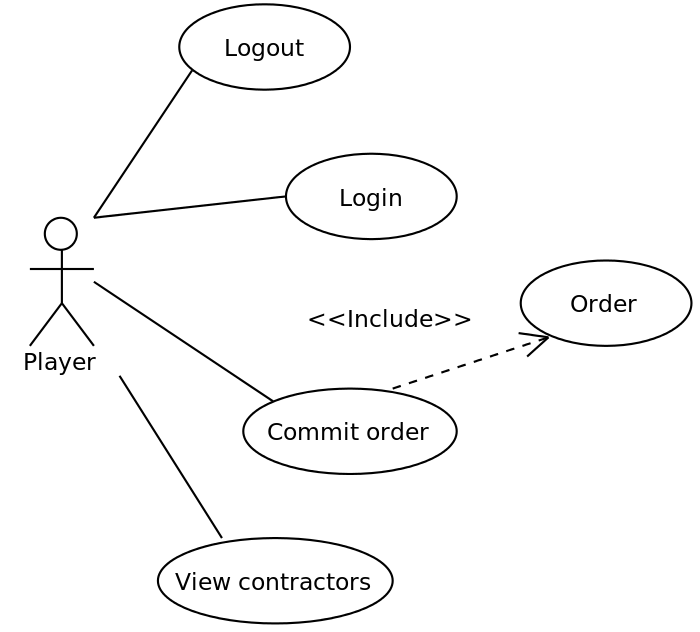
\includegraphics[width=3.5in]{images/uml/player_use_cases.png}
    \caption{Діаграма використання для гравця}
    \label{fig:uml_pl_uc}
\end{stdfigure}   

\begin{stdfigure}
    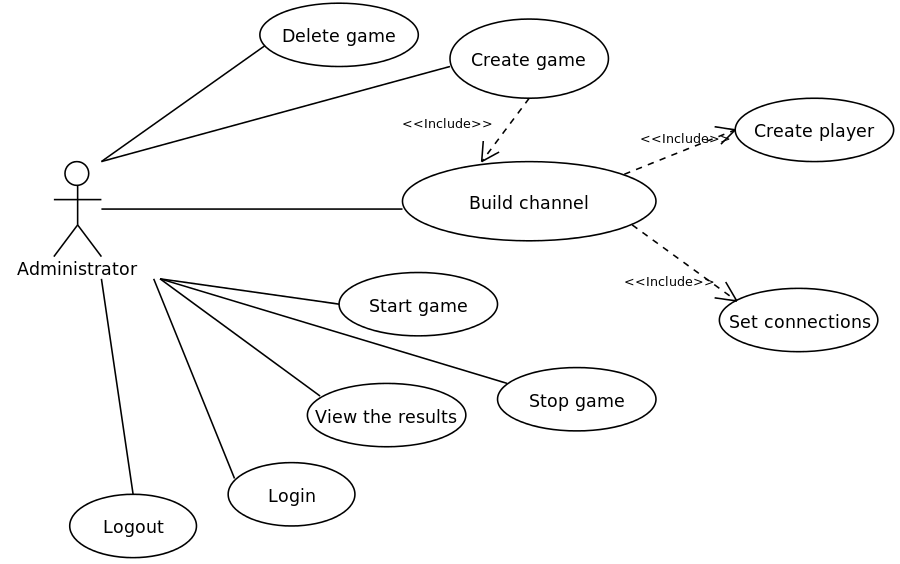
\includegraphics[width=6in]{images/uml/admin_use_cases.png}
    \caption{Діаграма використання для адміністратора}
    \label{fig:uml_admin_uc}
\end{stdfigure}
%3.4 Инструкция пользователю (описать с экранными формами как надо работать с программой)
\subsection{Інформаційно-логічна схема даних}
ER-модель --- це модель даних, яка дозволяє узагальнено описувати реляційну базу даних. На рис. \ref{fig:er} представлена логічна модель даних для розроблюваної системи.

%3.2 Информационно-логическая схема данных (ЕР модель)
\begin{stdfigure}
    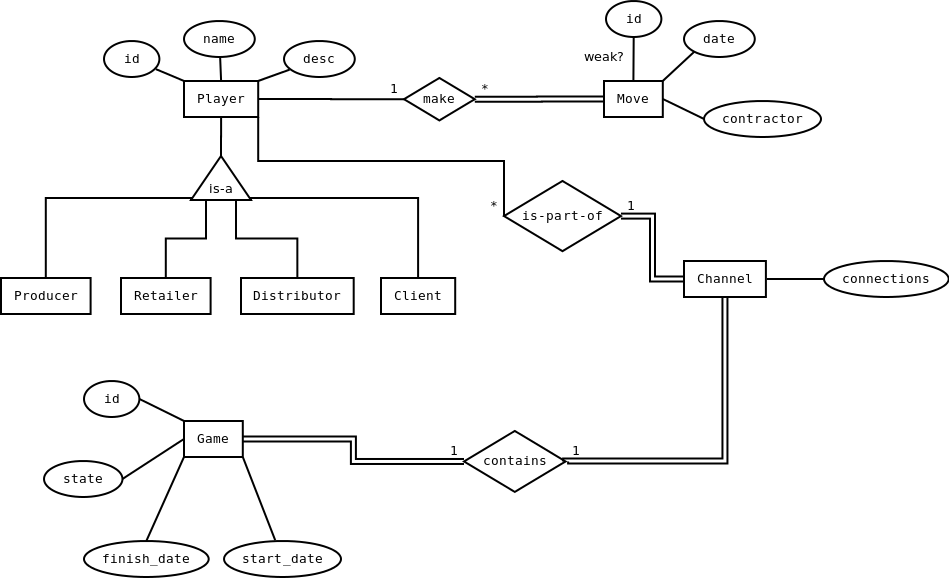
\includegraphics[width=7in]{images/er.png}
    \caption{Логічна модель даних}
    \label{fig:er}
\end{stdfigure}   

\subsection{Системна архітектура}
Система керування бізнес-грою розділена на п’ять базових компонентів (див. рис. \ref{fig:uml_components}): 
\begin{itemize}
\item тонкий веб-клієнт;
\item компонент, що керує обліковими записами, іграми, обслуговує запити користувачів;
\item компонент, що відподвідає за симуляцію як таку, за виконання логіки автоматичних гравців;
\item база даних, що обслуговує запити користувача;
\item оперативна база даних для моделювання;
\end{itemize}

Таке розділення на компоненти дозволяє розподілити навантаження по різних вузлах таким чином, щоби симуляція, що може потребувати значних ресурсів, не заважала коректній роботі системи з користувачами.
\begin{stdfigure}
    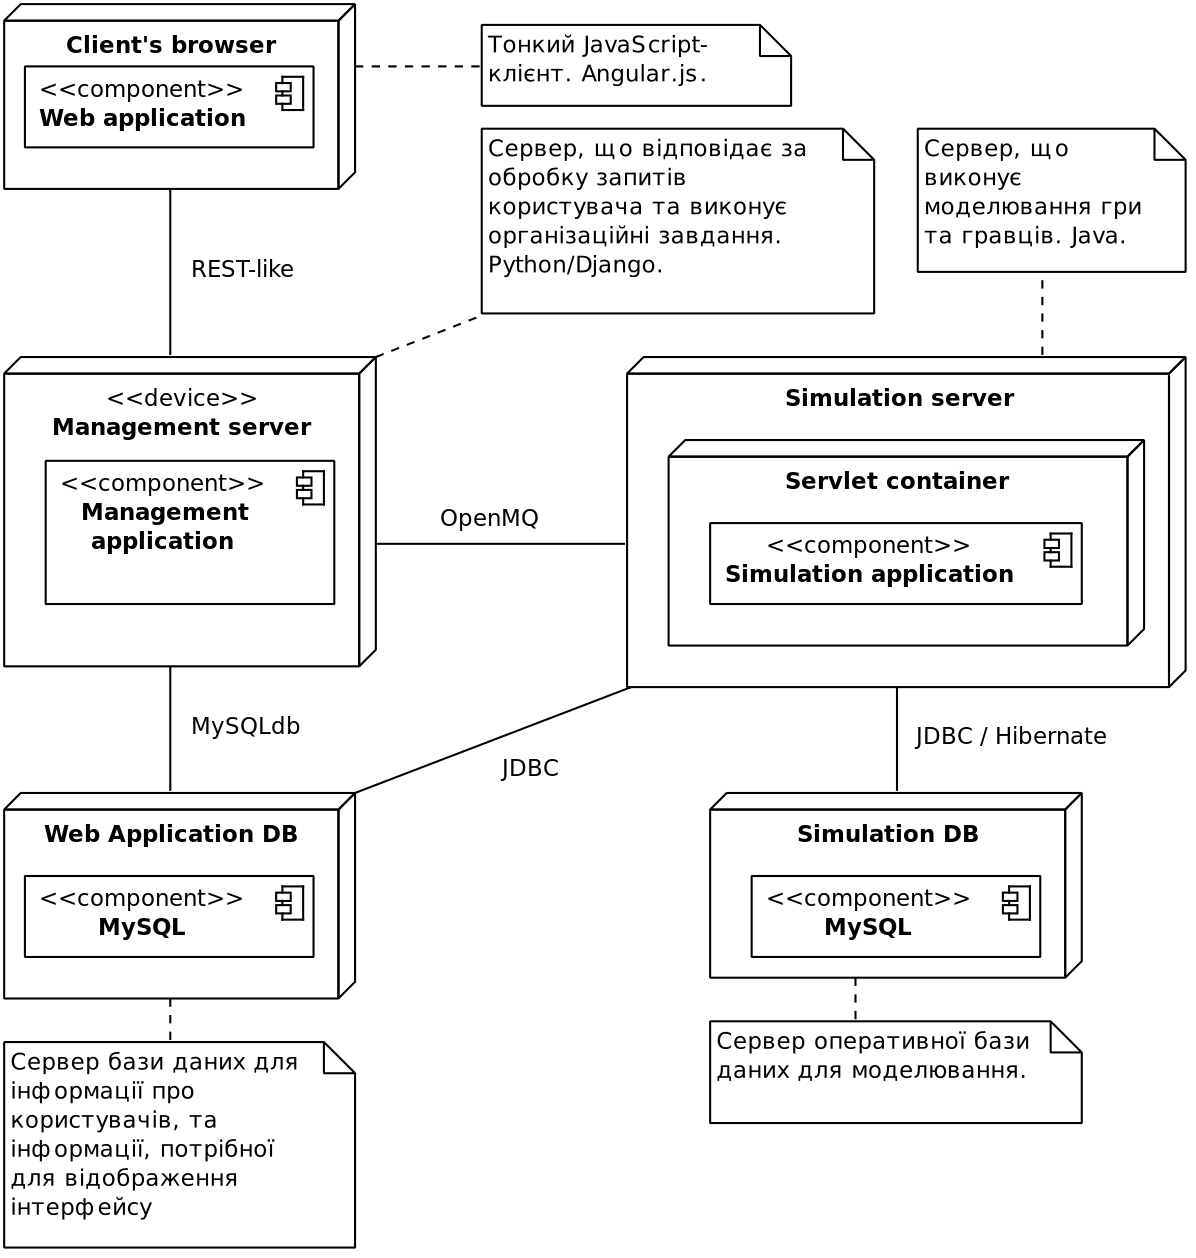
\includegraphics[width=4.5in]{images/uml/component_diagram.png}
    \caption{Діаграма розгортання}
    \label{fig:uml_components}
\end{stdfigure}   

Також були розроблені дві діаграми класів, що відображають загальну структуру двох компонентів: Management application та Simulation application. Як можна побачити на рис. \ref{fig:uml_management}, перший відповідає за взаємодію з користувачем та керування іграми, тоді як другий (див. рис. \ref{fig:uml_simulation}) відповідає за реалізацію імітаційної моделі та проведення експерементів.

\begin{stdfigure}
    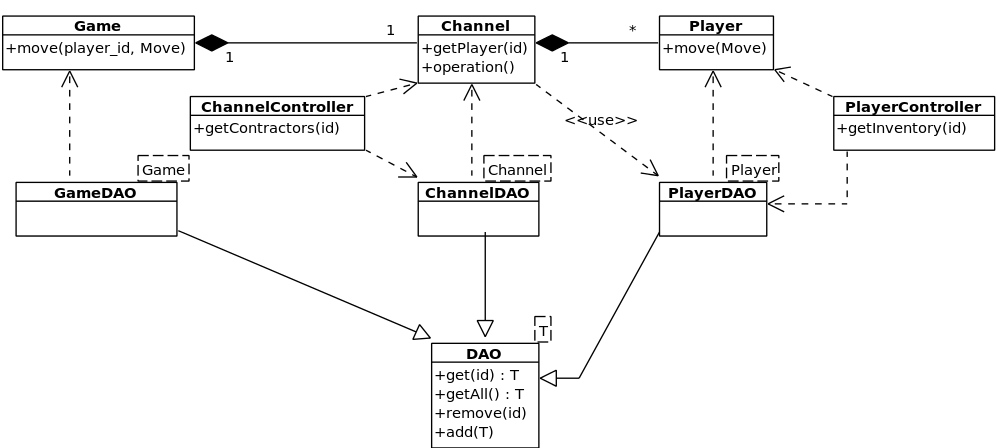
\includegraphics[width=7in]{images/uml/management_level.png}
    \caption{Діаграма класів Management Level}
    \label{fig:uml_management}
\end{stdfigure}   

\begin{stdfigure}
    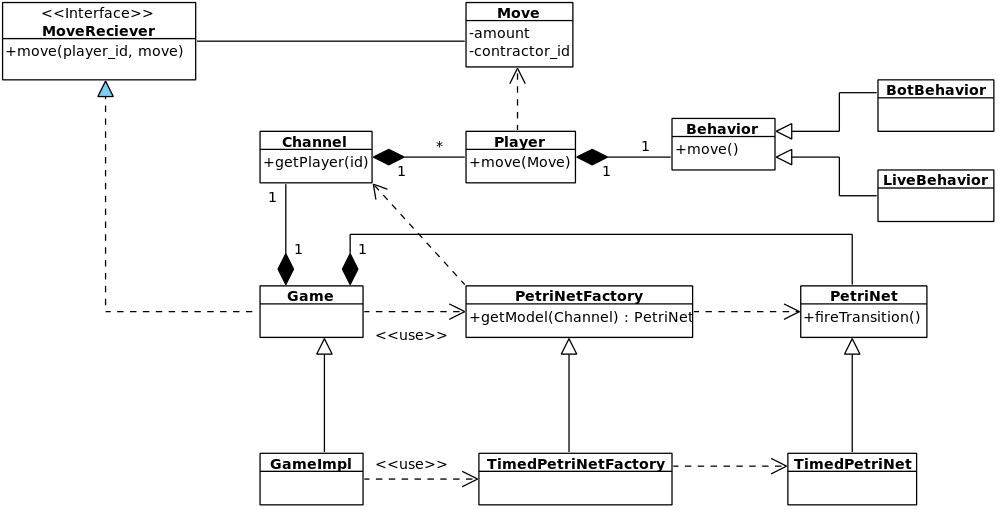
\includegraphics[width=7in]{images/uml/simulation_level.png}
    \caption{Діаграма класів Simulation Level}
    \label{fig:uml_simulation}
\end{stdfigure}   

\subsection{Алгоритмічне забезпечення}
Для розроблюваної системи були розроблені дві діаграми послідовностей (див. рис. \ref{fig:uml_live_move} та рис. \ref{fig:uml_auto_move}), що відображають алгоритми виконування ходу гравцем, якщо гравець реальний, та грою, якщо гравець є автоматичним.
\begin{stdfigure}
    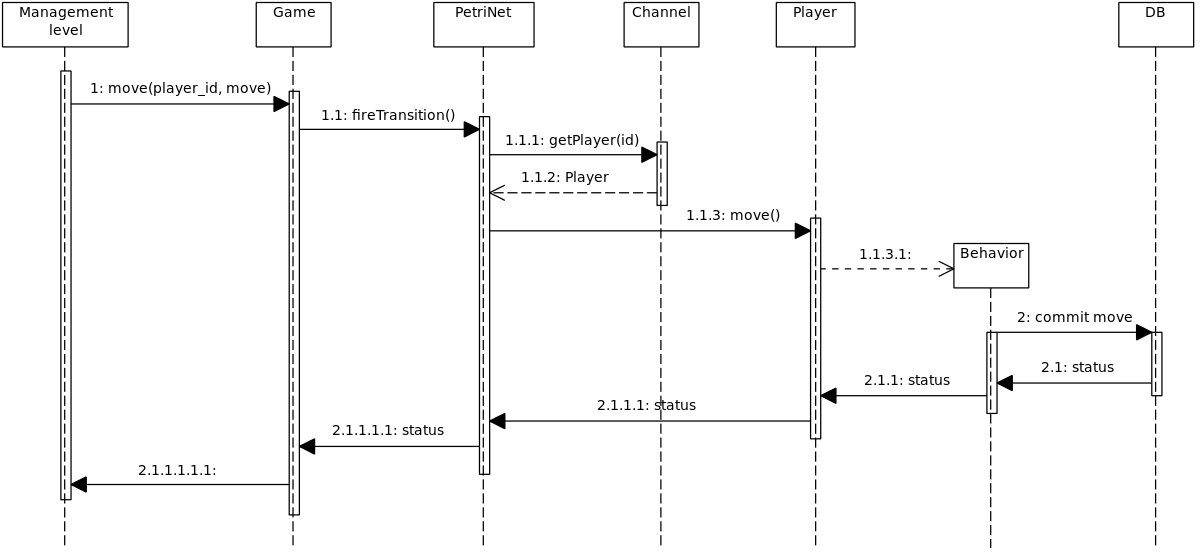
\includegraphics[width=7in]{images/uml/live_move.png}
    \caption{Діаграма послідовностей ходу реального гравця}
    \label{fig:uml_live_move}
\end{stdfigure}   

\begin{stdfigure}
    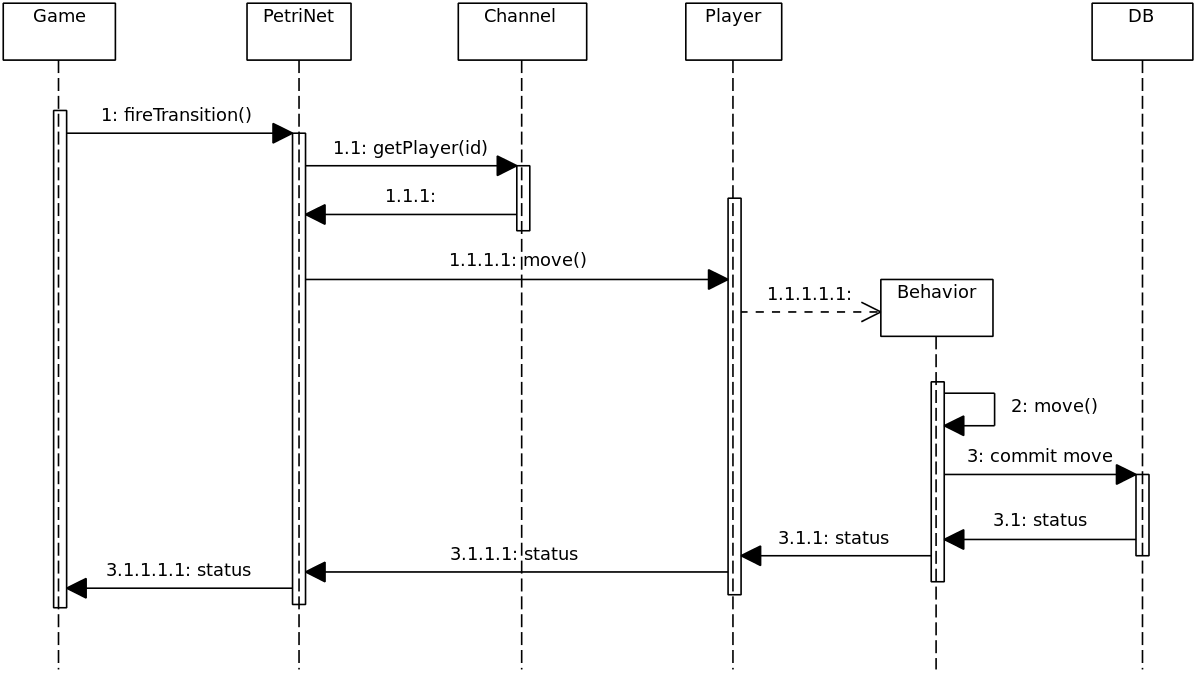
\includegraphics[width=7in]{images/uml/automate_move.png}
    \caption{Діаграма послідовностей ходу автоматичного гравця}
    \label{fig:uml_auto_move}
\end{stdfigure}   
%3.3 Алгоритмическое обеспечение (активити диаграммы)

\subsection{Інструкція користувача}
Робота з розробленою системою починається зі сторінки авторизації (рис. \ref{fig:login_screen}), з якої можна потрапити на екран гри (рис. \ref{fig:game_screen}) та на головну сторінку (рис. \ref{fig:main_screen}). З головної сторінки можна потрапити на сторінку з результатами роботи системи (\ref{fig:plot_screen}) та на сторінку гри. 

На екрані гри зображені у вигляді зеленого прямокутника контрагенти, доступні для замовлення. Щоб зробити замовлення, треба ввести кількість товару в текстове поле, натиснути кнопку <<Замовити>>. Після цього, замовлення повинно з’явитися в таблиці замовлень (як на рис. \ref{fig:step_screen}). Після того необхідно натиснути пункт меню <<Відправити>>. Після відправки замовлення можливі зміни в полі <<Запаси>>, якщо в системі спрацювали алгоритми автоматичних гравців.
\begin{stdfigure}
    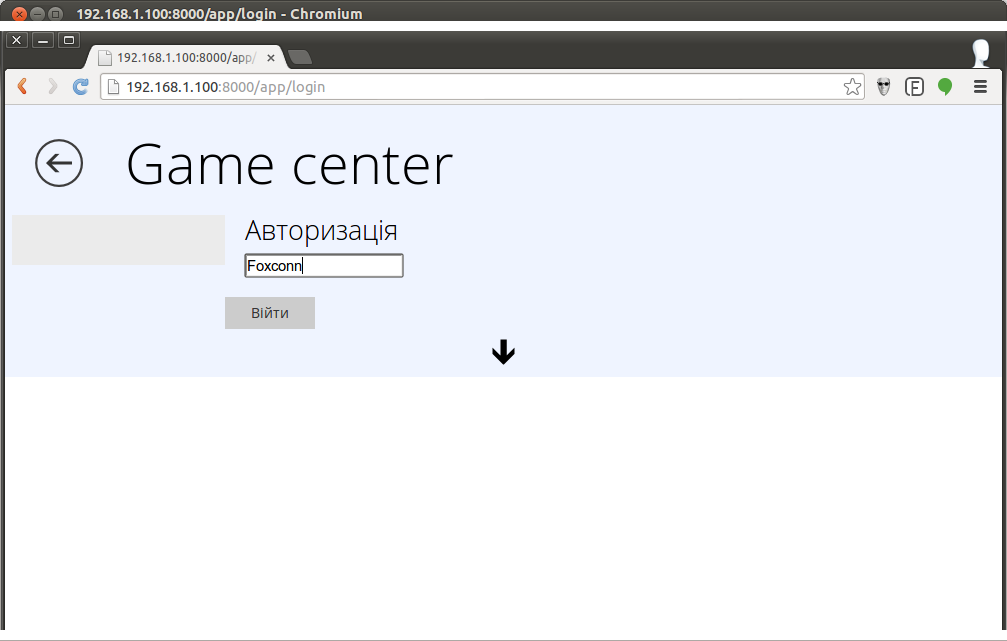
\includegraphics[width=7in]{images/screen/login_screen.png}
    \caption{Екран авторизації}
    \label{fig:login_screen}
\end{stdfigure}   
\begin{stdfigure}
    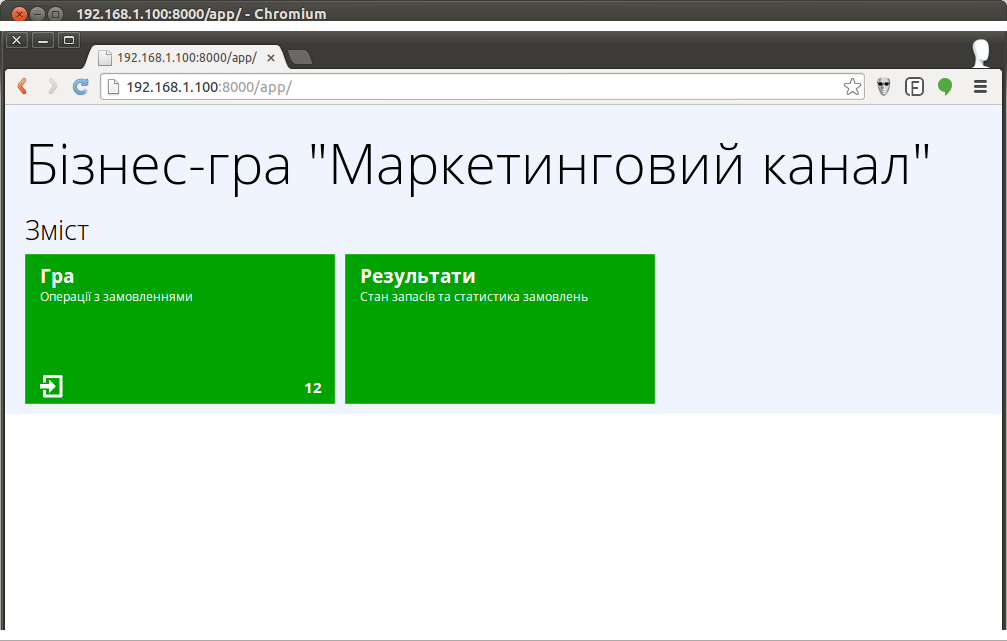
\includegraphics[width=7in]{images/screen/main_screen.png}
    \caption{Головний екран}
    \label{fig:main_screen}
\end{stdfigure}
\begin{stdfigure}
    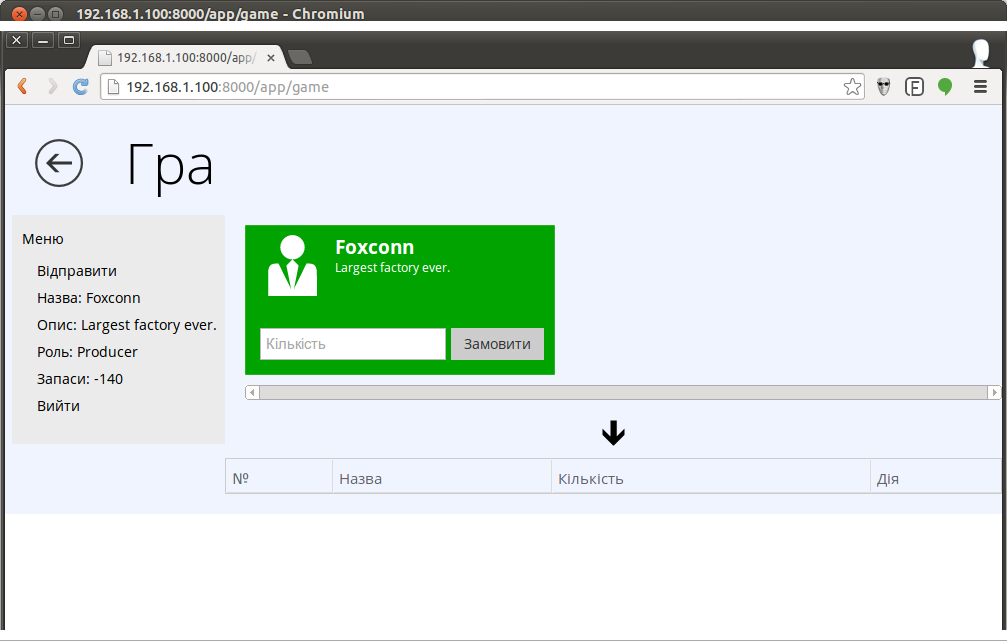
\includegraphics[width=7in]{images/screen/game_screen.png}
    \caption{Сторінка гри}
    \label{fig:game_screen}
\end{stdfigure}   
\begin{stdfigure}
    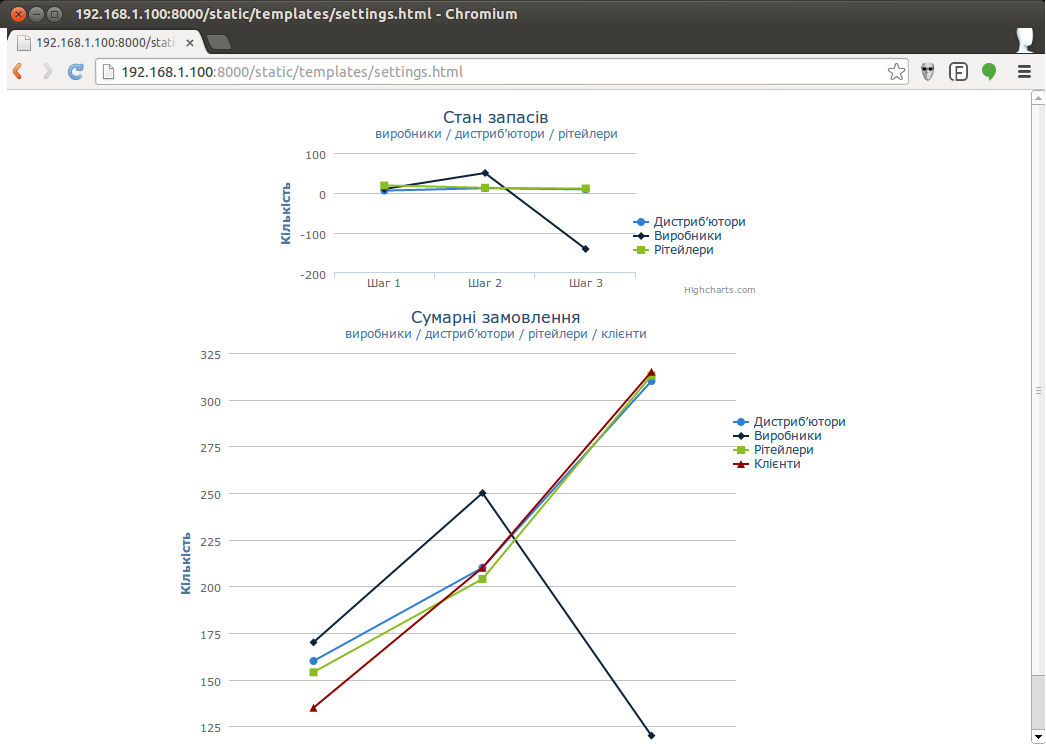
\includegraphics[width=7in]{images/screen/plot_screen.png}
    \caption{Сторінка результатів}
    \label{fig:plot_screen}
\end{stdfigure}   
\begin{stdfigure}
    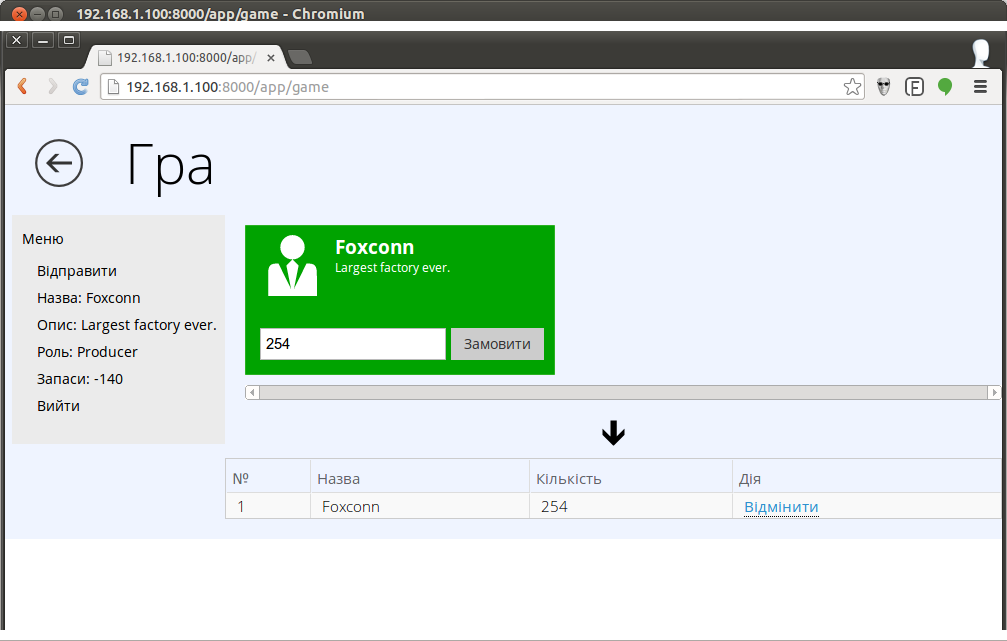
\includegraphics[width=7in]{images/screen/step_screen.png}
    \caption{Екран зі зробленим замовленням}
    \label{fig:step_screen}
\end{stdfigure}   
